\documentclass[tikz,border=5pt]{standalone}
\pdfinfoomitdate=1
\pdftrailerid{}
\pdfsuppressptexinfo=-1
\usepackage{pgfplots}
\usepgfplotslibrary{groupplots}
\pgfplotsset{compat=1.18}
\definecolor{atlasBlue}{HTML}{0072B2}
\definecolor{atlasOrange}{HTML}{E69F00}
\definecolor{atlasPurple}{HTML}{CC79A7}
\definecolor{atlasSky}{HTML}{56B4E9}
% NATO SERS F48; data_sha256=095874841672de0891d3b093d2959593e75f644fec4db3f593d64570b646304a
% (P) RQ-P01; M01 spectrum BA; points are domains; intervals resample physical masters.
\begin{document}
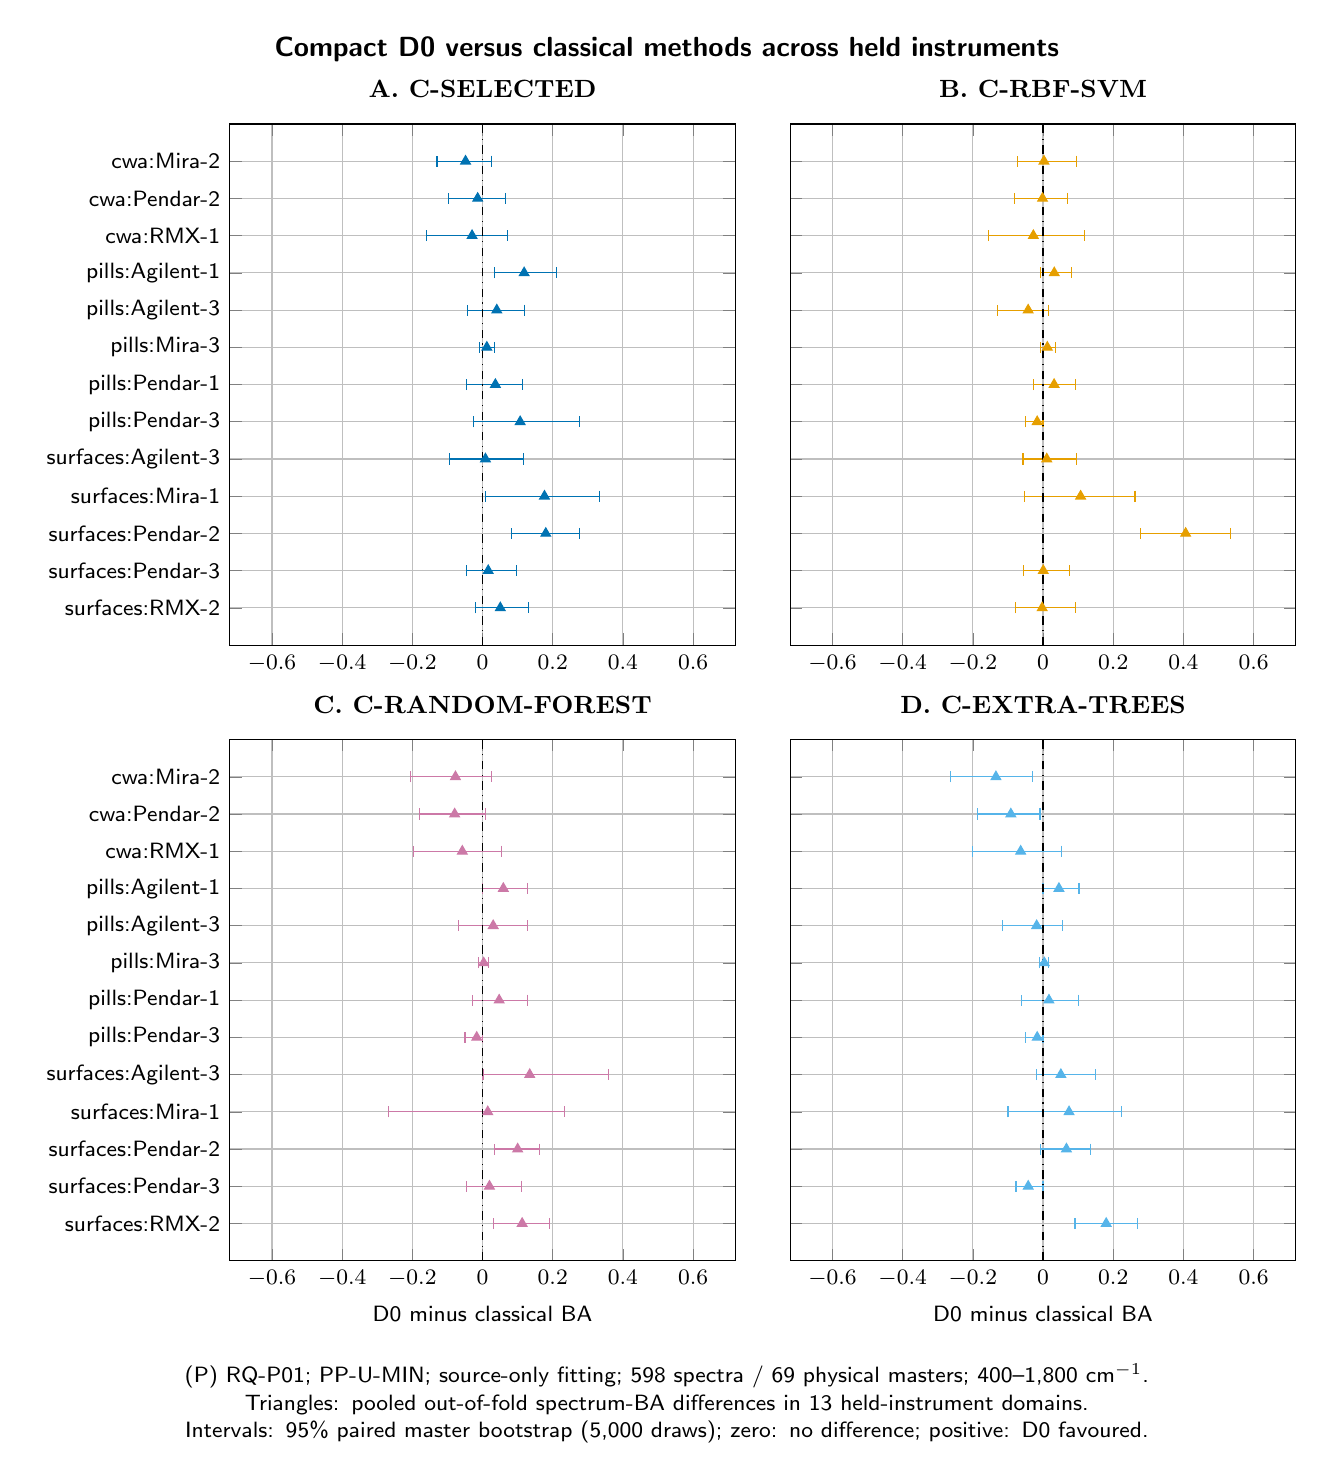
\begin{tikzpicture}
\begin{groupplot}[group style={group size=2 by 2,horizontal sep=0.7cm,vertical sep=1.2cm},width=8.0cm,height=8.2cm,grid=major,tick label style={font=\sffamily\fontsize{8}{10}\selectfont},label style={font=\sffamily\fontsize{8}{10}\selectfont},title style={font=\small\bfseries},y tick label style={align=right}]
\nextgroupplot[title={A. C-SELECTED},xlabel={},xmin=-0.72,xmax=0.72,ymin=-1,ymax=13,ytick={12,11,10,9,8,7,6,5,4,3,2,1,0},yticklabels={cwa:Mira-2,cwa:Pendar-2,cwa:RMX-1,pills:Agilent-1,pills:Agilent-3,pills:Mira-3,pills:Pendar-1,pills:Pendar-3,surfaces:Agilent-3,surfaces:Mira-1,surfaces:Pendar-2,surfaces:Pendar-3,surfaces:RMX-2}]
\addplot+[only marks,mark=triangle*,color=atlasBlue,mark options={fill=atlasBlue,draw=atlasBlue},error bars/.cd,x dir=both,x explicit] coordinates {(-0.048492063,12) += (0.074894324,0) -= (0.081263251,0) (-0.013984127,11) += (0.078357556,0) -= (0.083943505,0) (-0.029878788,10) += (0.10052435,0) -= (0.13064172,0) (0.11848485,9) += (0.091849086,0) -= (0.084790404,0) (0.040559441,8) += (0.077906036,0) -= (0.082983683,0) (0.012215054,7) += (0.022602954,0) -= (0.021697593,0) (0.036574074,6) += (0.078199705,0) -= (0.081812169,0) (0.10714286,5) += (0.16904762,0) -= (0.13253968,0) (0.0082010582,4) += (0.10763327,0) -= (0.10305225,0) (0.17643098,3) += (0.15690236,0) -= (0.16691353,0) (0.18015152,2) += (0.09704807,0) -= (0.096969697,0) (0.016130952,1) += (0.081488095,0) -= (0.062575397,0) (0.050574713,0) += (0.08016166,0) -= (0.071698126,0)};
\addplot[black,dashdotted] coordinates {(0,-1) (0,13)};
\nextgroupplot[title={B. C-RBF-SVM},xlabel={},xmin=-0.72,xmax=0.72,ymin=-1,ymax=13,ytick={12,11,10,9,8,7,6,5,4,3,2,1,0},yticklabels={}]
\addplot+[only marks,mark=triangle*,color=atlasOrange,mark options={fill=atlasOrange,draw=atlasOrange},error bars/.cd,x dir=both,x explicit] coordinates {(0.0026190476,12) += (0.092937308,0) -= (0.074159831,0) (-0.0014603175,11) += (0.071477762,0) -= (0.079861865,0) (-0.027636364,10) += (0.14498081,0) -= (0.12791919,0) (0.031969697,9) += (0.050304293,0) -= (0.038636364,0) (-0.042424242,8) += (0.056876457,0) -= (0.088060088,0) (0.012215054,7) += (0.022991142,0) -= (0.020611044,0) (0.031547619,6) += (0.060953477,0) -= (0.05911335,0) (-0.016666667,5) += (0.016666667,0) -= (0.033333333,0) (0.010582011,4) += (0.085717593,0) -= (0.067724868,0) (0.10707071,3) += (0.15483405,0) -= (0.15947547,0) (0.40636364,2) += (0.12818326,0) -= (0.12858586,0) (0.00063492063,1) += (0.075555556,0) -= (0.056725198,0) (-0.0024904215,0) += (0.09500935,0) -= (0.075899651,0)};
\addplot[black,dashdotted] coordinates {(0,-1) (0,13)};
\nextgroupplot[title={C. C-RANDOM-FOREST},xlabel={D0 minus classical BA},xmin=-0.72,xmax=0.72,ymin=-1,ymax=13,ytick={12,11,10,9,8,7,6,5,4,3,2,1,0},yticklabels={cwa:Mira-2,cwa:Pendar-2,cwa:RMX-1,pills:Agilent-1,pills:Agilent-3,pills:Mira-3,pills:Pendar-1,pills:Pendar-3,surfaces:Agilent-3,surfaces:Mira-1,surfaces:Pendar-2,surfaces:Pendar-3,surfaces:RMX-2}]
\addplot+[only marks,mark=triangle*,color=atlasPurple,mark options={fill=atlasPurple,draw=atlasPurple},error bars/.cd,x dir=both,x explicit] coordinates {(-0.077222222,12) += (0.10374248,0) -= (0.12898973,0) (-0.079470899,11) += (0.086600918,0) -= (0.10083128,0) (-0.05769697,10) += (0.1125331,0) -= (0.14030043,0) (0.059242424,9) += (0.068537879,0) -= (0.060454545,0) (0.03030303,8) += (0.097104377,0) -= (0.098316498,0) (0.0031827957,7) += (0.013710869,0) -= (0.014677049,0) (0.047354497,6) += (0.080287439,0) -= (0.075969285,0) (-0.016666667,5) += (0.016666667,0) -= (0.033333333,0) (0.13439153,4) += (0.22435305,0) -= (0.13318326,0) (0.014814815,3) += (0.21851852,0) -= (0.28317791,0) (0.1,2) += (0.061904762,0) -= (0.066666667,0) (0.01968254,1) += (0.091428571,0) -= (0.065395082,0) (0.11283525,0) += (0.078378315,0) -= (0.08160097,0)};
\addplot[black,dashdotted] coordinates {(0,-1) (0,13)};
\nextgroupplot[title={D. C-EXTRA-TREES},xlabel={D0 minus classical BA},xmin=-0.72,xmax=0.72,ymin=-1,ymax=13,ytick={12,11,10,9,8,7,6,5,4,3,2,1,0},yticklabels={}]
\addplot+[only marks,mark=triangle*,color=atlasSky,mark options={fill=atlasSky,draw=atlasSky},error bars/.cd,x dir=both,x explicit] coordinates {(-0.13420635,12) += (0.10464184,0) -= (0.12840522,0) (-0.091746032,11) += (0.083109858,0) -= (0.095394508,0) (-0.063757576,10) += (0.11713908,0) -= (0.13635528,0) (0.04530303,9) += (0.057294192,0) -= (0.04530303,0) (-0.018181818,8) += (0.073737374,0) -= (0.098484848,0) (0.0036989247,7) += (0.01111589,0) -= (0.013575468,0) (0.016798942,6) += (0.083302342,0) -= (0.079021164,0) (-0.016666667,5) += (0.016666667,0) -= (0.033333333,0) (0.050793651,4) += (0.097691198,0) -= (0.07049062,0) (0.074074074,3) += (0.15,0) -= (0.17407407,0) (0.066666667,2) += (0.069447464,0) -= (0.073015873,0) (-0.042222222,1) += (0.042222222,0) -= (0.034700855,0) (0.17998084,0) += (0.089697583,0) -= (0.088767571,0)};
\addplot[black,dashdotted] coordinates {(0,-1) (0,13)};

\end{groupplot}
\node[font=\sffamily\bfseries,anchor=south] at (current bounding box.north) {Compact D0 versus classical methods across held instruments};
\node[font=\sffamily\fontsize{8}{10}\selectfont,anchor=north,align=center,text width=16cm] at ([yshift=-3mm]current bounding box.south) {(P) RQ-P01; PP-U-MIN; source-only fitting; 598 spectra / 69 physical masters; 400--1,800 cm$^{-1}$.\\Triangles: pooled out-of-fold spectrum-BA differences in 13 held-instrument domains.\\Intervals: 95\% paired master bootstrap (5,000 draws); zero: no difference; positive: D0 favoured.};
\end{tikzpicture}
\end{document}
